\subsection{Introduction}
Image data provides an incredible resource for information extraction in disaster 
scenarios \cite{}



The first challenge is understanding how to utilize image data. One simple method would be to use 
a pre-trained multilabel classifier that includes 'Flood' as one of its labels. 

AWS Rekognition provides one such pre-trained classifier through its \textbf{detect\_labels} api. Classifying all the pictures in the Jakarta dataset (4900 images) 
reveals that 1600 of them have 
a 'Flood' label that has a confidence score of greater than .5. 

On the surface that seems promising, but plotting the results shows that using only 
this one feature creates a dataset that is not linearly separable. Adding more 
labels from the image classification, thus increasing the size of the feature space, 
will help us to differentiate between images that depict heavy flooding and those that 
are pointing out light flooding or clogged drains such as \ref{fig:clogged_drain}.

Perhaps we can choose labels that we think might be important- for example, 
maybe heavy flooding means that there won't be vehicles on the road so we can 
add the 'Vehicle' label. Or maybe we think that there might be 'Cars' but not 'Motorcycles' 
during heavy flooding. 

How do we go about choosing which labels are best?
If we train a classifier on the entirety of the data, and then see which classes have 
the most weight on the separator then we can find which labels are the most useful in 
separating flooding from non flooding images. 
\\
Carrying out this process using the perceptron algorithm shows that the 10 most important classes are: 

['Planter', 'Slum', 'Strap', 'Sedan', 'Grove', 'Parade', 'Ground', 'Vacation', 'Coupe', 'Trail']

\subsection{Evaluation}
The separator created by perceptron has an average .80 percent test success rate at classifying heavy 
flooding images from both datasets. 

\begin{figure}[ht]
    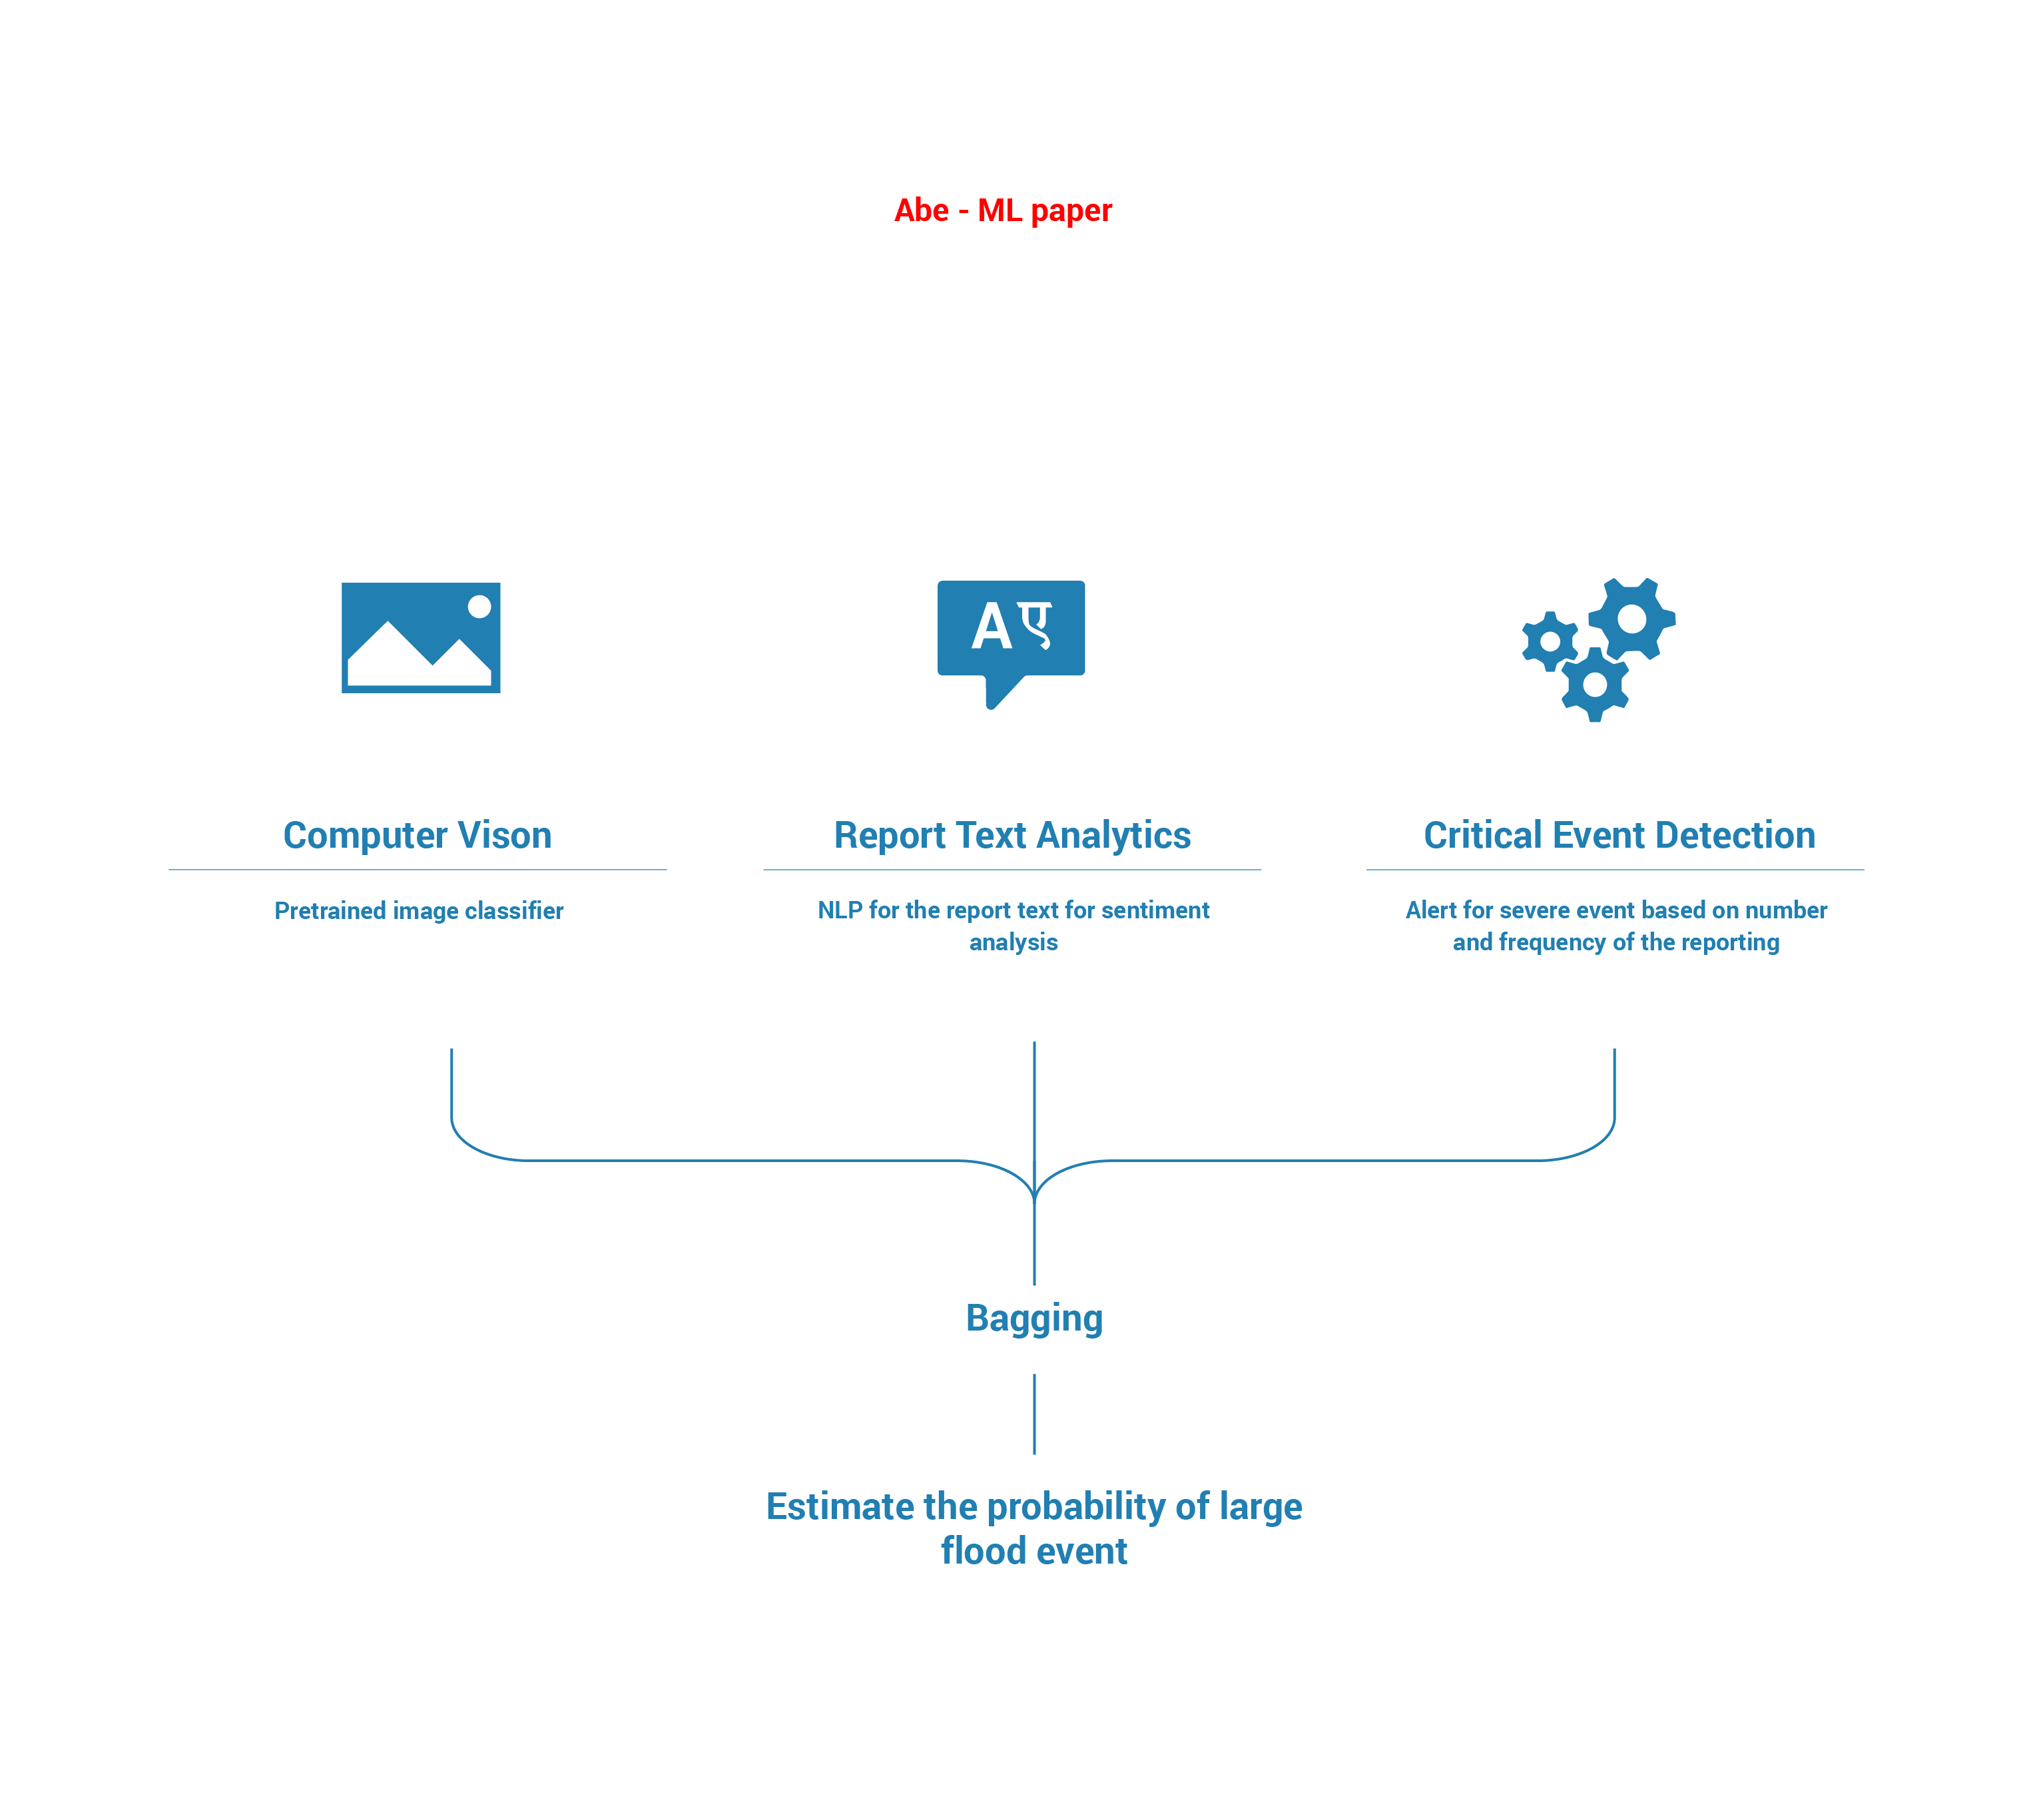
\includegraphics[width = 85mm]{ml_diagram.png}
    \caption{bagging}
    \label{fig:bagging}
\end{figure}